\documentclass[tikz,border=12pt]{standalone}
\usepackage[no-math]{fontspec}
\usepackage{xeCJK}
\usepackage[UTF8,fontset=none]{ctex}
\usepackage{tikz}
\usetikzlibrary{arrows.meta,positioning,fit,calc,backgrounds}

\IfFontExistsTF{Times New Roman}{\setmainfont{Times New Roman}}{\setmainfont{TeX Gyre Termes}}
\IfFontExistsTF{Kaiti TC}{\setCJKmainfont[AutoFakeBold=3]{Kaiti TC}}
  {\IfFontExistsTF{Songti TC}{\setCJKmainfont[AutoFakeBold=3]{Songti TC}}
    {\setCJKmainfont{PingFang TC}}}

% thesis_colors.tex ─ 論文統一 TikZ 色票定義
% 在每個 standalone 圖的 preamble 以 % thesis_colors.tex ─ 論文統一 TikZ 色票定義
% 在每個 standalone 圖的 preamble 以 % thesis_colors.tex ─ 論文統一 TikZ 色票定義
% 在每個 standalone 圖的 preamble 以 \input{thesis_colors.tex} 引入

\definecolor{thesisBlue}{RGB}{43,108,176}      % 訓練集、主箭頭、主色
\definecolor{thesisAmber}{RGB}{201,140,30}     % 驗證集、次要強調
\definecolor{thesisCrimson}{RGB}{155,35,53}    % 測試集、警示
\definecolor{thesisTeal}{RGB}{74,157,143}      % 節點類型 1（電子零組件）
\definecolor{thesisForest}{RGB}{45,122,79}     % 節點類型 2（光電及I/O）、LSTM Update
\definecolor{thesisSand}{RGB}{194,168,120}     % 節點類型 3（半導體）
\definecolor{thesisDark}{RGB}{45,55,72}        % 框線、文字、主箭頭
\definecolor{thesisLight}{RGB}{237,242,247}    % 淡背景、節點填色
\definecolor{thesisPurple}{RGB}{107,70,193}    % GAT 第二注意力頭
\definecolor{thesisMidGray}{RGB}{130,145,160}  % 次要線段、虛線
 引入

\definecolor{thesisBlue}{RGB}{43,108,176}      % 訓練集、主箭頭、主色
\definecolor{thesisAmber}{RGB}{201,140,30}     % 驗證集、次要強調
\definecolor{thesisCrimson}{RGB}{155,35,53}    % 測試集、警示
\definecolor{thesisTeal}{RGB}{74,157,143}      % 節點類型 1（電子零組件）
\definecolor{thesisForest}{RGB}{45,122,79}     % 節點類型 2（光電及I/O）、LSTM Update
\definecolor{thesisSand}{RGB}{194,168,120}     % 節點類型 3（半導體）
\definecolor{thesisDark}{RGB}{45,55,72}        % 框線、文字、主箭頭
\definecolor{thesisLight}{RGB}{237,242,247}    % 淡背景、節點填色
\definecolor{thesisPurple}{RGB}{107,70,193}    % GAT 第二注意力頭
\definecolor{thesisMidGray}{RGB}{130,145,160}  % 次要線段、虛線
 引入

\definecolor{thesisBlue}{RGB}{43,108,176}      % 訓練集、主箭頭、主色
\definecolor{thesisAmber}{RGB}{201,140,30}     % 驗證集、次要強調
\definecolor{thesisCrimson}{RGB}{155,35,53}    % 測試集、警示
\definecolor{thesisTeal}{RGB}{74,157,143}      % 節點類型 1（電子零組件）
\definecolor{thesisForest}{RGB}{45,122,79}     % 節點類型 2（光電及I/O）、LSTM Update
\definecolor{thesisSand}{RGB}{194,168,120}     % 節點類型 3（半導體）
\definecolor{thesisDark}{RGB}{45,55,72}        % 框線、文字、主箭頭
\definecolor{thesisLight}{RGB}{237,242,247}    % 淡背景、節點填色
\definecolor{thesisPurple}{RGB}{107,70,193}    % GAT 第二注意力頭
\definecolor{thesisMidGray}{RGB}{130,145,160}  % 次要線段、虛線


% Node colors cycling for input/output feature nodes
\colorlet{nc1}{thesisTeal}
\colorlet{nc2}{thesisCrimson}
\colorlet{nc3}{thesisAmber}
\colorlet{nc4}{thesisPurple}
\colorlet{nc5}{thesisForest}

\begin{document}
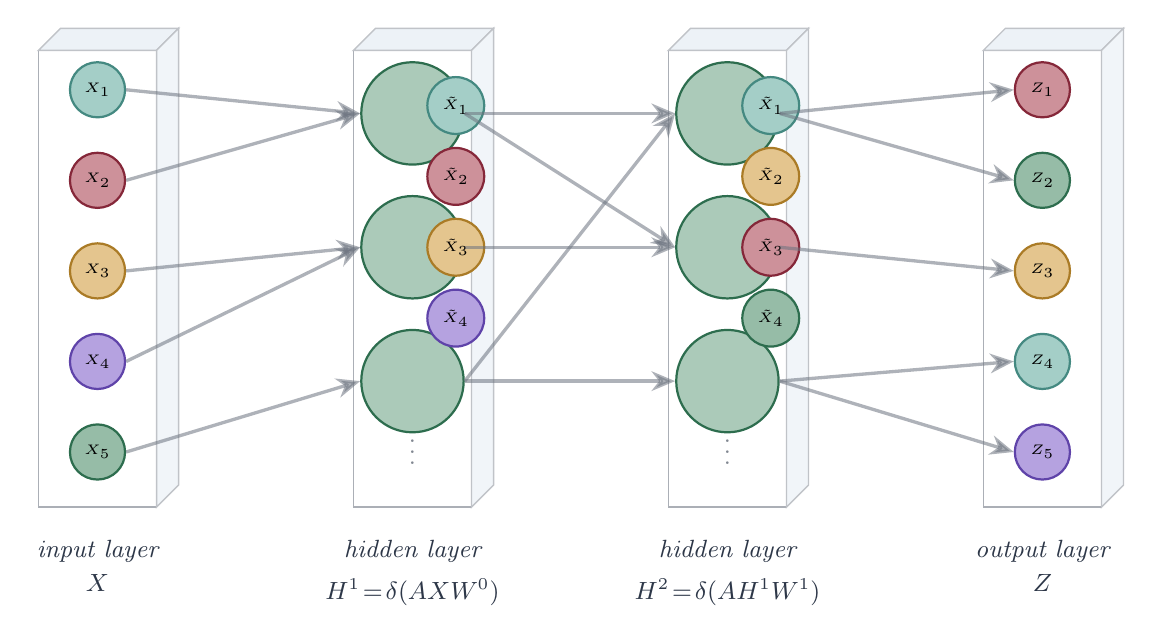
\begin{tikzpicture}[
  bignode/.style={circle, draw=thesisForest!80!thesisDark, fill=thesisForest!40,
                  thick, minimum size=13mm},
  smallnode/.style={circle, draw=#1!80!thesisDark, fill=#1!50, thick, minimum size=7mm},
  arr/.style={-{Stealth[length=3mm,width=2.5mm]}, thesisDark!70, line width=1.2pt},
  layerlabel/.style={font=\small\itshape, thesisDark},
  eqlabel/.style={font=\small, thesisDark, align=center},
]

\def\sep{4.0}    % horizontal spacing between layers
\def\vsep{1.15}  % vertical spacing between nodes within layer
\def\depth{0.28} % 3-D offset depth
\def\lw{1.5}     % layer panel width
\def\lh{5.8}     % layer panel height

% ─── helper macro: draw one layer column ───────────────────────
% #1=x-center, #2=y-top, #3=panel label text, #4=number of feature nodes
\newcommand{\drawlayer}[4]{%
  \begin{pgfonlayer}{background}
    % front face (white, slight border)
    \fill[white, draw=thesisDark!40, line width=0.6pt]
         ({#1-\lw/2},{#2-\lh}) rectangle ({#1+\lw/2},{#2});
    % top face (light gray parallelogram)
    \fill[thesisLight, draw=thesisDark!30, line width=0.5pt]
         ({#1-\lw/2},{#2}) -- ({#1-\lw/2+\depth},{#2+\depth})
         -- ({#1+\lw/2+\depth},{#2+\depth}) -- ({#1+\lw/2},{#2}) -- cycle;
    % right face (light gray parallelogram)
    \fill[thesisLight!80, draw=thesisDark!30, line width=0.5pt]
         ({#1+\lw/2},{#2}) -- ({#1+\lw/2+\depth},{#2+\depth})
         -- ({#1+\lw/2+\depth},{#2-\lh+\depth}) -- ({#1+\lw/2},{#2-\lh}) -- cycle;
  \end{pgfonlayer}
}

% ─── Layer 0: Input X ──────────────────────────────────────────
\def\x{0}
\drawlayer{\x}{4.5}{}{5}
\node[layerlabel, below] at (\x, -1.6) {input layer};
\node[layerlabel, below=1pt] at (\x, -2.0) {$X$};

% Feature nodes in layer 0
\foreach \row/\col in {1/nc1, 2/nc2, 3/nc3, 4/nc4, 5/nc5}{
  \node[smallnode=\col] (x\row) at (\x, {4.0 - (\row-1)*\vsep})
      {\tiny $X_{\row}$};
}

% ─── Layer 1: H^1 ──────────────────────────────────────────────
\def\x{\sep}
\drawlayer{\x}{4.5}{}{4}
\node[layerlabel, below] at (\x,-1.6) {hidden layer};
\node[eqlabel, below=1pt] at (\x,-2.05)
    {$H^1\!=\!\delta(AXW^0)$};

% Big green aggregation nodes
\foreach \row in {1,2,3}{
  \node[bignode] (h1big\row) at (\x, {3.7 - (\row-1)*1.7}) {};
}
% Small feature nodes (lighter)
\foreach \row/\col in {1/nc1, 2/nc2, 3/nc3, 4/nc4}{
  \node[smallnode=\col, minimum size=5mm] (h1s\row) at ({\x+0.55}, {3.8-(\row-1)*0.9})
      {\tiny $\tilde{X}_{\row}$};
}
% dots
\node[font=\small, thesisDark!60] at (\x, -0.5) {$\vdots$};

% ─── Layer 2: H^2 ──────────────────────────────────────────────
\def\x{2*\sep}
\drawlayer{\x}{4.5}{}{4}
\node[layerlabel, below] at (\x,-1.6) {hidden layer};
\node[eqlabel, below=1pt] at (\x,-2.05)
    {$H^2\!=\!\delta(AH^1W^1)$};

\foreach \row in {1,2,3}{
  \node[bignode] (h2big\row) at (\x, {3.7 - (\row-1)*1.7}) {};
}
\foreach \row/\col in {1/nc1, 2/nc3, 3/nc2, 4/nc5}{
  \node[smallnode=\col, minimum size=5mm] (h2s\row) at ({\x+0.55}, {3.8-(\row-1)*0.9})
      {\tiny $\tilde{X}_{\row}$};
}
\node[font=\small, thesisDark!60] at (\x,-0.5) {$\vdots$};

% ─── Layer 3: Output Z ─────────────────────────────────────────
\def\x{3*\sep}
\drawlayer{\x}{4.5}{}{5}
\node[layerlabel, below] at (\x,-1.6) {output layer};
\node[layerlabel, below=1pt] at (\x,-2.0) {$Z$};

\foreach \row/\col in {1/nc2, 2/nc5, 3/nc3, 4/nc1, 5/nc4}{
  \node[smallnode=\col] (z\row) at (\x, {4.0-(\row-1)*\vsep})
      {\tiny $Z_{\row}$};
}

% ─── Layer-to-layer arrows (batch, sampled) ─────────────────────
\foreach \fr/\to in {x1/h1big1, x2/h1big1, x3/h1big2, x4/h1big2, x5/h1big3}{
  \draw[arr, opacity=0.55] (\fr.east) -- (\to.west);
}
\foreach \fr/\to in {h1big1/h2big1, h1big2/h2big2, h1big3/h2big3,
                     h1big1/h2big2, h1big3/h2big1}{
  \draw[arr, opacity=0.55] (\fr.east) -- (\to.west);
}
\foreach \fr/\to in {h2big1/z1, h2big1/z2, h2big2/z3, h2big3/z4, h2big3/z5}{
  \draw[arr, opacity=0.55] (\fr.east) -- (\to.west);
}

\end{tikzpicture}
\end{document}
